\documentclass[a4paper,12pt]{report}

\usepackage[utf8]{inputenc}
\usepackage{amsmath}
\usepackage{fontspec}
\usepackage{float}
\usepackage{enumitem}
\usepackage{graphicx}
\usepackage{wrapfig}
\usepackage{setspace}
\usepackage[titletoc]{appendix}
\usepackage{pdfpages} 
\usepackage{cite}
\usepackage{url}
\usepackage{listings}
\usepackage{color}

\definecolor{codegreen}{rgb}{0,0.6,0}
\definecolor{codegray}{rgb}{0.5,0.5,0.5}
\definecolor{codepurple}{rgb}{0.58,0,0.82}

\lstdefinestyle{mystyle}{
	backgroundcolor=\color{white},   
	commentstyle=\color{codegreen},
	keywordstyle=\color{blue},
	numberstyle=\tiny\color{codegray},
	stringstyle=\color{codepurple},
	basicstyle=\footnotesize,
	breakatwhitespace=false,         
	breaklines=true,                 
	captionpos=b,                    
	keepspaces=true,                 
	numbers=left,                    
	numbersep=5pt,                  
	showspaces=false,                
	showstringspaces=false,
	showtabs=false,                  
	tabsize=2
}

\lstset{style=mystyle}

\setlength{\parindent}{0em}
\setlength{\parskip}{0.5em}

\setmainfont[
BoldFont=arialbd.ttf,
ItalicFont=ariali.ttf,
BoldItalicFont=arialbi.ttf
]{arial.ttf}

\author{Arundathi Shaji Shanthini}


\renewcommand{\bibname}{References}

%\setlength{\voffset}{-0.75in}

\begin{document}
%%%%%%%%%%%COVERSHEET%%%%%%%%%%%%%%%%%
\begin{titlepage}
    \setlength{\voffset}{-1.8in}
    \noindent \noindent \makebox[\textwidth]{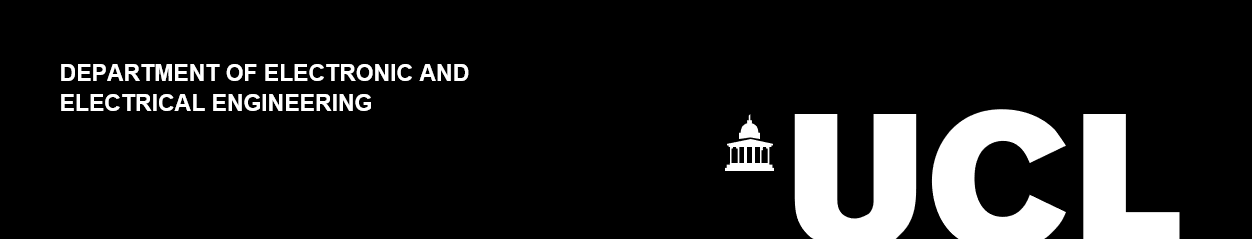
\includegraphics[width=1.55\textwidth]{images/Coversheet_Header_black_with_text.png}}
    
    \vspace{30mm}

    \begin{center}
        {\LARGE \textbf{BEng Project}}\\
        \vspace{4mm}
        {\Huge \textbf{Interim Report}}
    \end{center}
    
    \vspace{10mm}
    
    \begin{center}
    \begin{spacing}{1.8}
    {\LARGE
   Dynamic Modelling of a Continuum Robotic Snake-arm and its Performance Evaluation by Analysing Robustness}
    \end{spacing}
    \end{center}
    
   \vspace{5mm}
    
     \begin{tabular}{ll}
        \textbf{Student Name:}  & \hspace{4mm} Arundathi Shaji Shanthini \\
       \textbf{Contact e-mail:} & \hspace{4mm} arundathi.shanthini.16@ucl.ac.uk \\
        \textbf{Student number:} & \hspace{4mm} 16018351 \\ \\ 
        \textbf{Project Supervisor:}  & \hspace{4mm} Prof. Sarah Spurgeon \\
        \textbf{Contact e-mail:}  & \hspace{4mm} s.spurgeon@ucl.ac.uk \\
         \textbf{Department:} & \hspace{4mm} Department of Electronic and Electrical Engineering\\ \\ 
          \textbf{Submission Date:} & \hspace{4mm} 13\textsuperscript{th} of December 2019
    \end{tabular}
\end{titlepage}
%%%%%%%%%%%%%%%%%%%%%%%%%%%%%%%%%%%%%%

\pagebreak

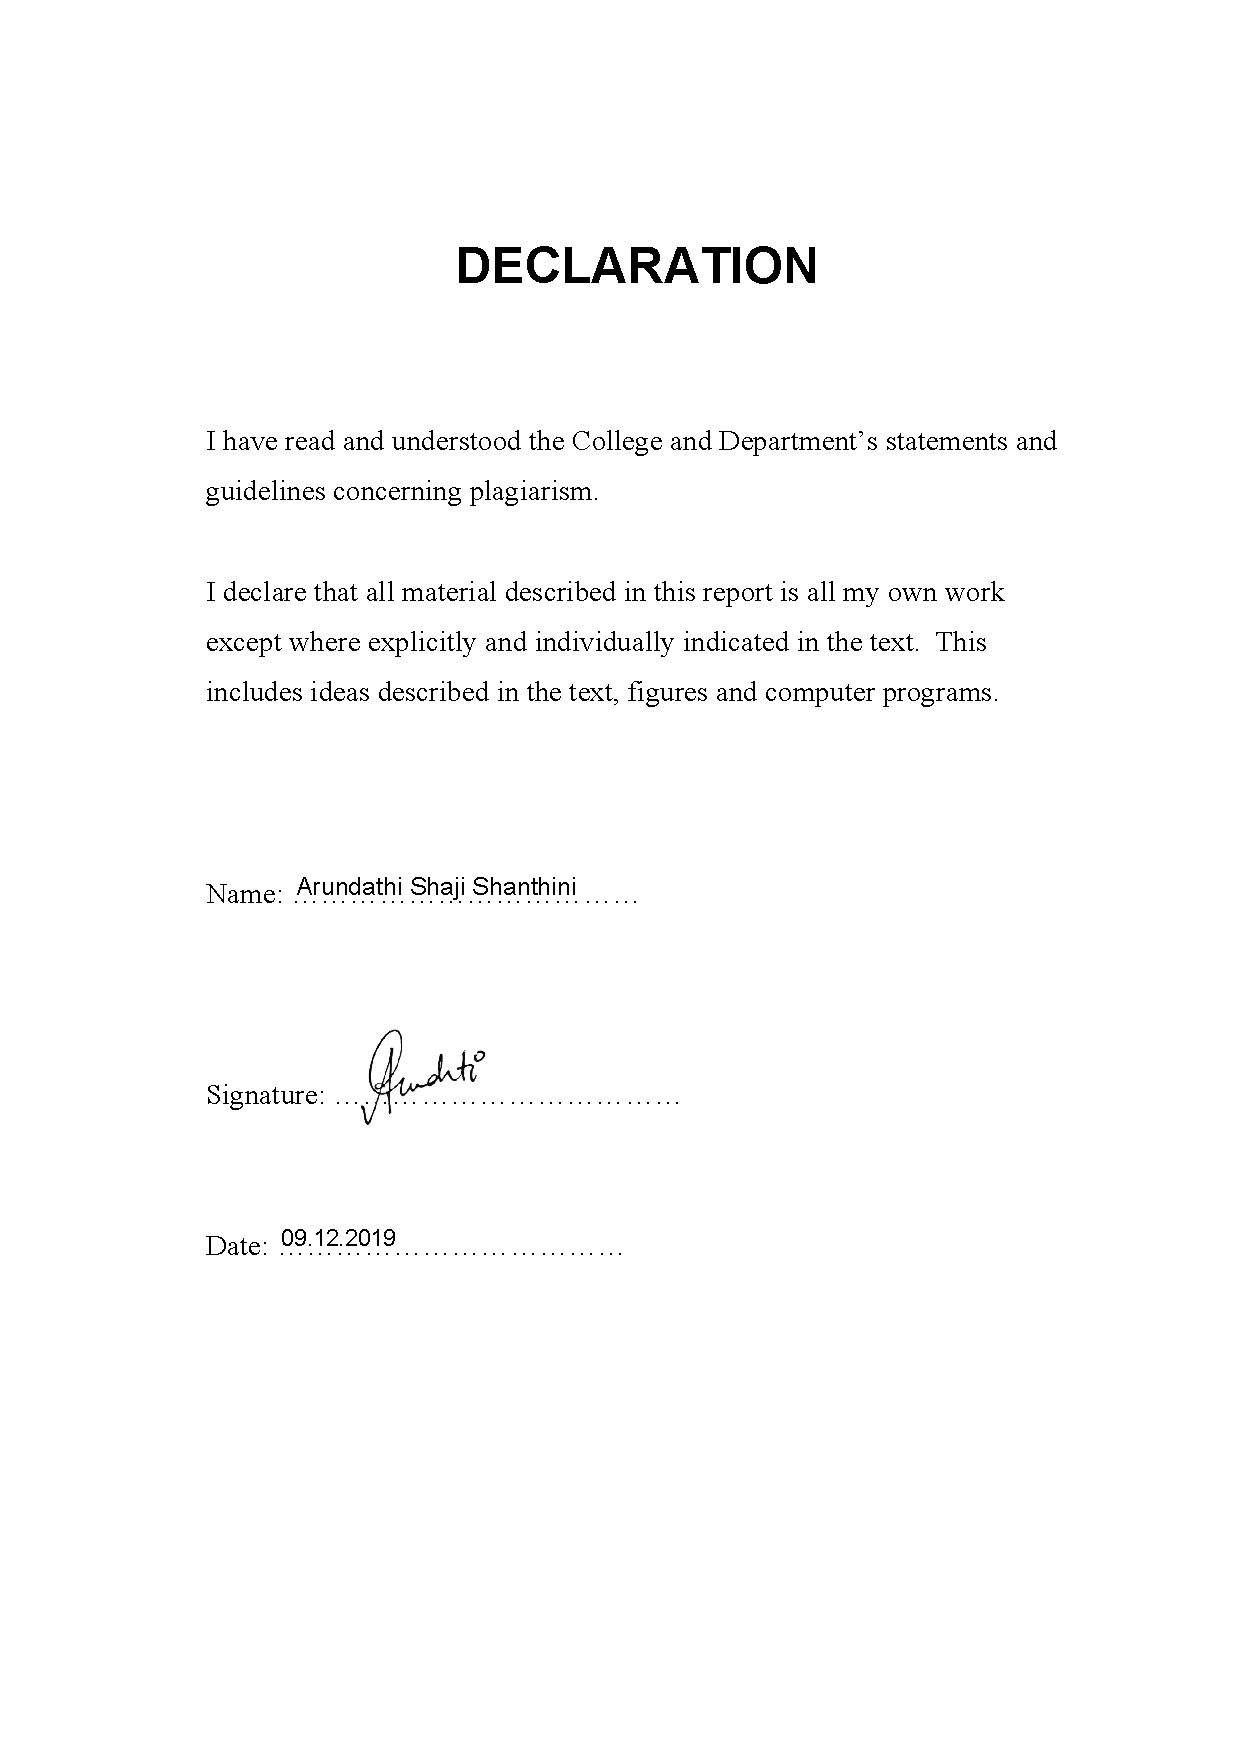
\includepdf[page=-]{files/Declaration}

\tableofcontents

\pagebreak

%%%%%%%%%%% ABSTRACT %%%%%%%%%%%%%%%%%
\begin{abstract}
    Cable-driven continuum robotic arms are widely used because of its very high accessibility and manoeuvrability properties and ability to perform dexterous in-situ tasks in confined spaces. However, for imaging/measurement applications achieving accurate end-effector pose becomes important. This project involves modelling such a system and developing a control configuration for it which is potentially robust. For this, the kinematic model of the system was studied and implemented using Simulink. Implementing the dynamic model and testing control configurations remain additional work to complete.
    
\end{abstract}
%%%%%%%%%%%%%%%%%%%%%%%%%%%%%%%%%%%%%%

%%%%%%%%%%% INTRODUCTION %%%%%%%%%%%%%%%%%
\chapter{Introduction}
\section{Project Description and Motivations}
Industrial robots that perform repetitive dexterous tasks have been around for quite some time. Over the years these industrial robots have developed from being just command following, space-occupying large devices to systems with better manoeuvrability, intelligence and accessibility properties that can perform a myriad of operations. Expanding a robot's workspace by improving the manoeuvrability of a robot has been of great interest and over the past decade a lot of interest has grown towards bio-mimetic or bio-inspired systems. Bio-inspired robotic systems involves studying concepts of locomotion from nature and implementing that into robotic systems. One such bio-inspired systems are snakebots. The locomotion achieved by snakes is highly desirable because of its accessibility and manoeuvrability properties which means that snakes can access confined spaces and manoeuver through different kinds of terrain.

This makes the robot very useful as it finds itself a wide range of applications such as disaster management (it can collect data and images from inaccessible areas at search and rescue sites), industrial inspection - like subsea operations, aircraft wing inspection, military reconnaissance etc. Figure \ref{snakebots-fig} shows some of the different kinds of snakebots that have been developed over the years by different research groups around the world.
\begin{figure}[h]
	\centering
	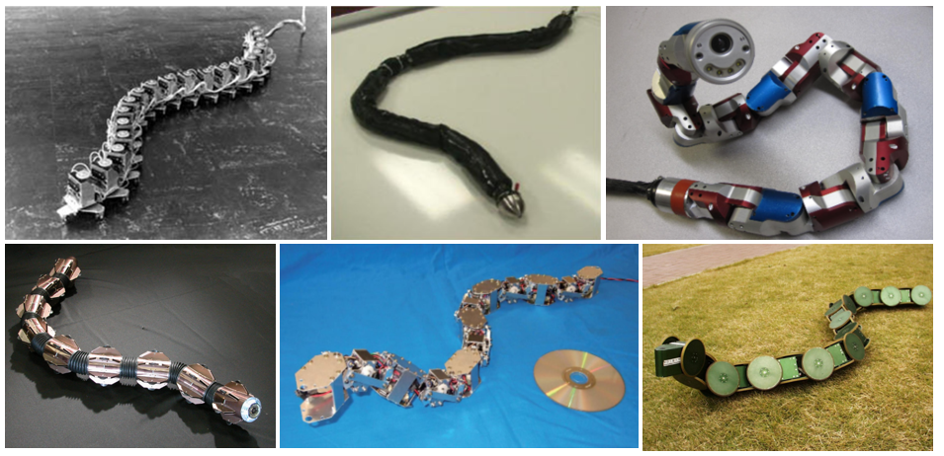
\includegraphics[width=\textwidth]{images/Intro-pic1.png}
	\caption{\textit{This picture shows some of the various kinds of snakebots that were developed over the years. It shows examples of wheeled, wheel-less and amphibious snakebots that have been developed. The pictures were sourced from a reveiw on snakebots by Liljeb{\"a}ck P. et.al. \cite{liljeback2012review}}}
	\label{snakebots-fig}
\end{figure}

While ground-hugging, vertebrae structure type snakebots are studied for their ability to propagate through challenging terrains, there are also studies around using the body-structure of snakes as an inspiration for developing wire-driven “invertebrate like” continuum robotic arms which have better flexibility and manoeuvrability. Continuum robotic arms are continuously curving manipulators that can be used to manoeuvre through confined and inaccessible places and can be made to perform dexterous in-situ tasks.


\begin{wrapfigure}{r}{0.6\textwidth}
	\centering
	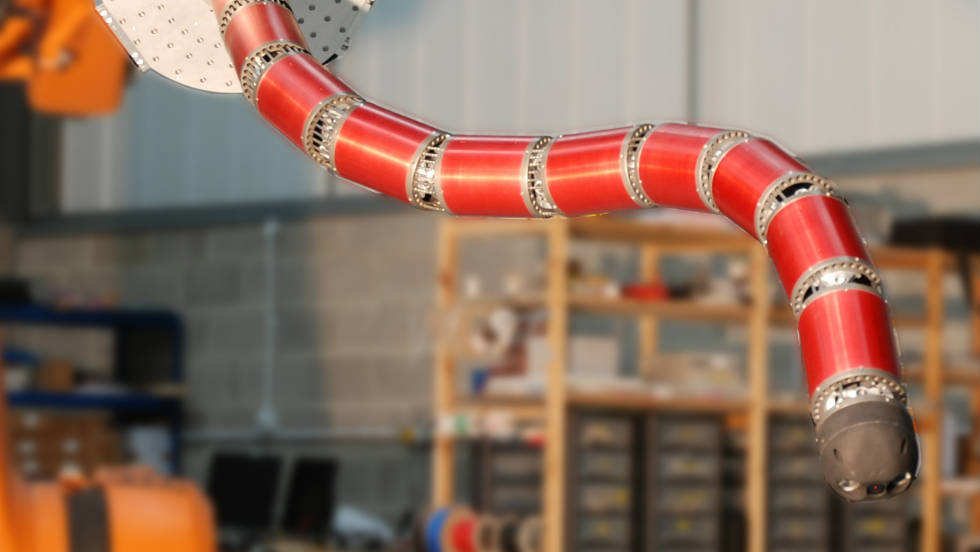
\includegraphics[width=0.6\textwidth]{images/CDHM.jpg}
	\caption{\textit{A cable-driven robotic snake arm developed by OC Robotics \cite{ CNNarticle}}}
\end{wrapfigure}

Cable-driven Hyper-redundant Manipulator (CDHRM) are one such kind of continuum robotic arms that are driven by wire-ropes and can be used in various applications involving service operations in confined spaces and hazardous environments, close range measurements, imaging etc. The main advantage of this particular kind of robotic arm is that, it has no electronics in the robot itself. All of the electronics associated with the robot is located in the base to which the arm is tethered. This makes it possible for the robot to access even hazardous environments without any risk of damage to the robot (except structural damage may occur in some cases) or hindrance to its operation. Such a structure makes risk assessments for the application of such a system in industry easier. 

Currently at UCL, a key area for research undertaken by the UCL Robotics Institute addresses one of the technology challenges of Robotics and Autonomous Systems (RAS) which is - “Robotic Teleoperation for Multiple Scales”. Under this challenge, attempts have been made to use photogrammetry techniques for the structural testing of aircraft wing of an Airbus by measuring the shape and dimensions of aerodynamic surfaces \cite{shortis2016photogrammetric}, and the six degrees of freedom (6DoF) position and orientation of aerospace models to study its structural dynamics and aerodynamic forces.

Photogrammetry is one of the optical metrology methods that obtains measurements of physical objects and/or their environment with a high accuracy through the process of capturing or recording photographic images and patterns of electromagnetic imagery and analysing it to measure and interpret reliable information of the object and environment under consideration. There are many variants of photogrammetry. The photogrammetry technique being studied at UCL involves the measurement of shape of aerodynamic surfaces and the six degree of freedom (6DoF) position and orientation of aerospace models.

Photogrammetry for aerospace models requires a non-contact, non-intrusive, accurate and reliable technique with a high sample rate. Within this study, the measurement of aerospace models in wind tunnel test sections are novel and for such a specialised measurement, close range photogrammetry is well suited. Currently off-the-shelf-digital cameras are used from different fixed positions to simultaneously capture/record images, however this has limitations and makes close-range photogrammetry difficult.

The proposed solution to this involves using a snake-arm that uses optical metrology techniques for aerodynamic surfaces. For this study, there is a physical snake-arm on-site at Here East and this project proposed is aligned to the modelling and control research effort being developed for this snakebot.

The snake-arm robot at Here East has been provided by OC Robotics. It is classified as Series II X125 snake-arm robot. The robot was specifically designed for the robotic deployment of photogrammetry capability for measurement and inspection of cluttered or confined 3D environments. This snake-arm is the unsleeved version of the Series II X125. It can potentially achieve up to 225 degrees of cumulative bend \cite{OCRobotics_Series_II_Webpage} and has an independently controlled tip. Currently, it simply uses a nose following control technique to reach to the desired final position.  The head of the snake can have different payloads attached to it. Unlike other versions of this series of snake-arms, the tethered end of this robot rests on a platform that can move forward and backward as required.

This project involves modelling this physical snakebot and understanding the end-effector pose control requirements for performing automated close-range optical metrology operations (specially photogrammetry). Once the control requirements are defined and the control strategies are realised, then the project aims to develop a robust control system that can perform measurements in various scenarios including measurements in wind tunnels. The control system configuration will be simulated, and the results obtained will be analysed and improved over the course of the project. Depending on the metrology technique adopted and in the case of using the robot to perform dexterous tasks such as maintenance of the structure, the payload attached to the head of the robot is subject to change. Significant external disturbances may be acting on the robot as well, especially in cases where the robot is performing dexterous tasks or is in environment with considerable disturbances like in a wind tunnel. Therefore, the robustness of the system will be tested using change in mass of head node and/or external disturbances acting on the snake-arm.

\section{Aims and Objectives}
\label{objectives}
The aim of this project is to contribute to the modelling and control effort around the snake-arm at Here East by developing and implementing a mathematical model and testing a control system configuration suitable for the task.

The main objectives of the project are:
\begin{itemize}
	\item \textbf{Develop and implement a mathematical model that best represents the snake-arm at Here East:} The main aim of the project is to develop and implement a mathematical model that best represents the system using Simulink. The model will be then tested to ensure that its behaviour is as expected and represents the snake-arm well.
	\item \textbf{Design and test control strategies that will help control the path followed by the arm during the metrology task:} The next objective is to define control requirements for the automation of the optical metrology process and design control strategies that performs the operation with the required accuracy. Through iterative testing, the model will be improved over the course of the project till satisfactory results are obtained.
	\item \textbf{Analyse the robustness of the control system configuration developed by running experiments with varied physical parameters:} The project also aims to investigate the robustness of the system since it is expected to work in environments with varied conditions where external disturbances affecting the arm’s propagation might be considerable. It is also expected that depending on the technique adopted for the optical metrology different payloads may be attached to the head of the snakebot. The payload may also change in mass especially in occasions when improvements have been made to the same metrology technique under consideration. Therefore, the robustness of the system under the influence of change of mass of the head and the external disturbances will be investigated through experiments in the simulation software.
\end{itemize}

\section{Literature Review}

On investigating some of the literature around snakebots it can be seen that many different kinds of approaches were adopted towards developing snakebots. Earlier in the decade, wheeled snakebots were being developed a lot more than wheel-less snakebots. \cite{saito2002modeling} discusses some of the very early work done on wheeled snake robots and gives more insight to the motivations for study of wheel-less snake robots. Hirose S. \cite{1521742} through his work came up with the mathematical equation that represented the shape that the snake assumes to propagate forward. He introduced the concept of serpenoid curve which has been extensively used by other research groups till date to develop a mathematical model for the serpentine locomotion of snakes. Work done by Pettersen, K. Y. et. al. \cite{pettersen2017snake} also provides a very detailed insight into the research around snake robots and discusses the mathematical model, design and control system used for productionising amphibious snake robots. This source is an excellent summary of the history and study of snake robots. While these most of these papers discuss wheel-less snake robots with rigid links, \cite{Zhou2018AnalysisOU} discusses how wire-driven "invertebrate like" continuum arm can have better flexibility and accessibility properties. A detailed review on the work done around continuum robots has also been published by Singh P. K. et. al.\cite{singh2014continuum}.


Since, the system under consideration is specifically that of the OC Robotics snake arm, materials published by the founders Graham A. and Buckingham R. were of immense interest. Even though material directly related to the robot or its technology could not be found, \cite{RN4,RN5,RN42} by these authors were a good introduction to their work on snake arms and the bigger context of the varied applications of such robots. The slides in \cite{RN42}, also discussed the main features of  snake arm robots.

Given that the system was identified as a wire rope driven, hollow core structure with passive revolute joints connecting the links to each other, attempts were made to identify literature around modelling of a similar system. The work of Jones B. et al. \cite{RN2} (dated 2006) has been cited in most papers. His work on kinematics for multi-section continuum robots seems to be the inspiration for most of the work around continuum snake arm robots. The works of Li Z. et al. \cite{RN8,RN7,RN15,RN21} discusses how the skeleton of the robot is inspired from the skeleton of a snake and the idea of a the cable driven structure is inspired from the muscle arrangement in the tentacle of an octopus. Even though across various papers their work discusses the kinematic model of the snake arm robot, they do not discuss much about the dynamic model and control of the system. The references \cite{RN35,RN31,RN29,RN30} represents the OC robotics snake arm the most. The system described by these papers uses a cable-driven hyper-redundant manipulator (CDHRM) in which the cables are controlled at the base with maxon motors exactly like the snake arm at Here East. The papers published by Tang L. et al. \cite{RN35,RN31} describes the design, motion planning and path tracking of the snake-arm.  However, the work of Xu W. et al \cite{RN30} dated 2018, remains the most suitable reference found so far as it discusses the dynamic model and control of the cable-driven snake arm in great detail. 

\vspace{20mm}

The following chapters discuss the progress made towards achieving the goals and objectives stated in this chapter. Chapter 2 discusses the mathematical model equations and its brief derivation. Chapter 3 discusses the first attempt at implementing the equations on Simulink and describes how they were cross-validated. Finally, Chapter 4 lists the summary of difficulties and issues faced and also discusses briefly the additional work to be done Term 2 to achieve the goals.


%%%%%%%%%%%%%%%%%%%%%%%%%%%%%%%%%%%%%%

%%%%%%%%%%% MATHEMATICAL MODELLING %%%%%%%%%%%%%%%%%
\chapter{Mathematical Modelling}
This chapter discusses mainly work done towards the tasks associated with the Preparatory phase (first phase) of the project. Whilst Literature review has already been discussed in the previous chapter, the chapter will mainly discuss the mathematical equations associated to kinematics of the snake-arm under consideration.
\section{Project Scheduling}
The Preparatory Phase ran for roughly 1.5 months of the project. Figure \ref{gc-1} shows the updated Gantt Chart\footnote{The old Gannt Chart has been added to Appendix \ref{appendix:a}} for these tasks. 
\begin{figure}[h]
	\centering
	\includegraphics[width=\textwidth]{images/GC-chap2.png}
	\caption{\textit{Gantt Chart showing tasks associated to Preparatory Phase}}
	\label{gc-1}
\end{figure}


\section{Understanding the system}
To find the most suitable mathematical model that suits the snake-arm, a clear understanding of the system itself was to be established. Understanding the actuators that drive the system and understanding what parameters can be controlled was also essential to determine what terms should be used to represent the mathematical model.

The videos that have been made available by OC Robotics specially \cite{OCRobotics_videos_1, OCRobotics_videos_2, OCRobotics_videos_3, OCRobotics_videos_4}, helped understand the snake-arm and its capabilities to an extent. The snake-arm developed by OC Robotics is a hollow core structure with a fixed number of links. Each link is driven by 3 wire ropes (big stainless steel cable ropes) runs through the case at equidistant points from each other parallel to the surface of the case outside it \cite{OCRobotics_article} (as can be seen in Figure \ref{base-pic}). The cables are controlled by 30 or more motors in the base \cite{OCRobotics_videos_2} using maxon mators as it offers higher power density. All the electronics associated to the robot including the control systems are located at the base of the robot. This means that the robot can easily operate in even hazardous environments. The nose of the snake arm can accommodate different payloads and given that the snake arm also has a hollow core, it thus allows cables, hoses or any other equipment required by the specific payload to be routed through the centre of the snake arm.
\begin{wrapfigure}{r}{0.6\textwidth}
	\centering
	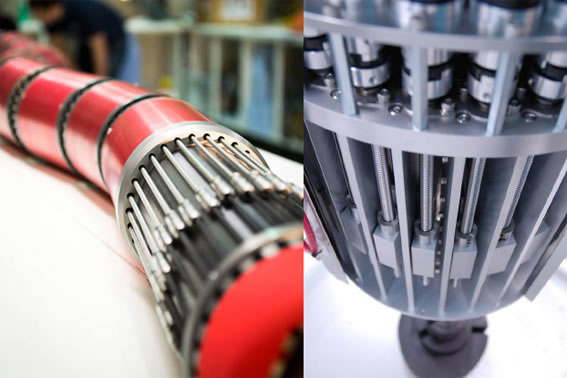
\includegraphics[width=0.6\textwidth]{images/maxon-motors.jpg}
	\caption{\textit{The figure showing the maxon motors at the base to which the wire-ropes are attached (right) and the transmission system (left) that converts the rotational motion of motor to translational motion of the wire-ropes. \cite{ CNNarticle}}}
	\label{base-pic}
\end{wrapfigure}
In the video for Maxon Motors \cite{OCRobotics_videos_2}, Graham A. also talks about the unique nose following property of the snake arm robot and how it is easily controlled using a proprietary software developed by OC Robotics. 
From these information, it can been safely concluded that the system closely represents a CDHRM and so the mathematical model developed for the robot was derived with help mainly from the following literature \cite{RN30, RN31, RN29} around modelling of a CDHRM. Kinematic modelling and Dynamic modelling have both been studied for the CDHRM. While kinematic modelling of the CDHRM has been thoroughly studied, there are only very few papers that discuss dynamic modelling.

\section{The Mathematical Model}
Consider a CDHRM snake-arm with \textbf{N universal joints} and hence has \textbf{N+1 links}. The length of each link is $a$ and the distance between the two links is $2d$. Each universal joint consists of 2 revolute joints connected via a common lumen which facilitate either a pitch or yaw rotation which imparts each joint 2 degrees of freedom (DoF). This means that in total the snake arm has \textbf{2N DoF}. 

Every link has an identical structure connected to each other at $90\circ$ with respect to each other. A link consists of a hollow cylindrical case with two identical disks consisting a revolute joint attached to both sides of the case. The links are arranged such that it forms a
\begin{wrapfigure}{r}{0.4\textwidth}
	\centering
	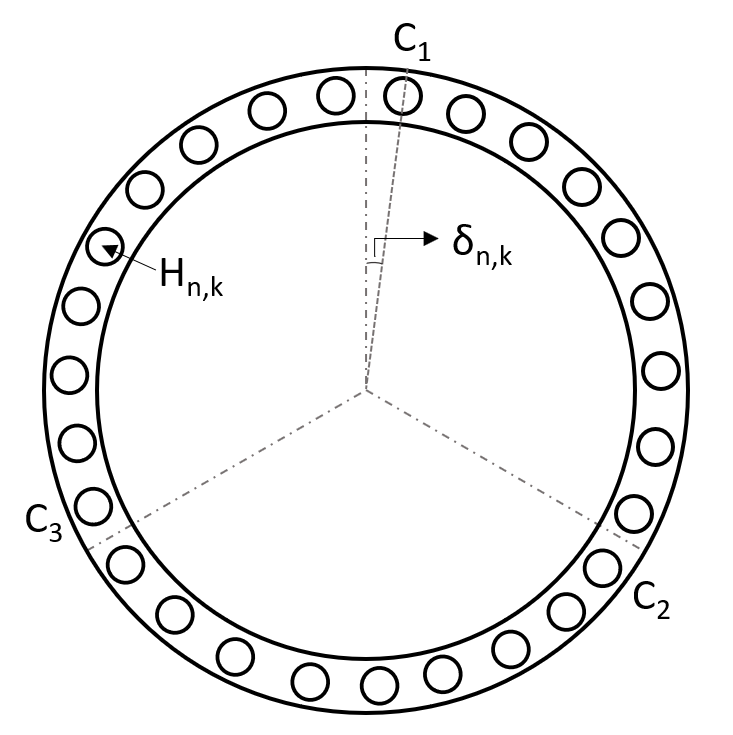
\includegraphics[width=0.4\textwidth]{images/hole_positions.png}
	\caption{\textit{This diagram shows the different reference frames that were defined}}
	\label{hole-pos}
\end{wrapfigure} 
\begin{center}
	Yaw) --- (Pitch-Yaw) --- (Yaw-Pitch) --- (Pitch-Yaw)\ldots\ldots) --- End-effector
\end{center} 
arrangement. For a given joint n, the disc attached to link n-1 is called the \textbf{distal disc} and the disc attached to link n is called the \textbf{proximal disc}. 

 Each link is driven by three cables. For a given link n, cables $C_{3n-2}$,$C_{3n-1}$ and $C_{3n}$ drive and terminate at the distal disc of the link. This means that for the cables to pass through, there are 3(N+1) holes\footnote{The link nearest to the base is fixed and cannot move. However, cables hold this link in place as well and hence we calculate number of holes as 3(N+1) instead of 3N. However note that in the cable length kinematic relations only 3N cables are considered since the three cables attached to the first link do not contribute to the formation of the joint angles and only 3N cables drive the robot.} on the discs attached to each link. The angular position of these holes as seen in Figure \ref{hole-pos} can be calculated as:
\begin{equation}
\delta_{k,n} =
\begin{cases}
\frac{360^{\circ}}{3(N+1)} \times ceil(k/3) +12(k-1) &; \hspace{3mm}  \text{if n=odd}   \\
\frac{360^{\circ}}{3(N+1)} \times ceil(k/3) +12(k-1) + 90 &; \hspace{3mm}  \text{if n=even}
\end{cases}
\end{equation}


\subsection{Kinematic Modelling}
The kinematic model which gives the relationship between the angle of rotation of the motor and the end-effector pose of the snake-arm is derived by multi-level mapping through relationships between parameters in different spaces. Figure \ref{kinematic map} below depicts this.
\begin{figure}[h]
	\centering
	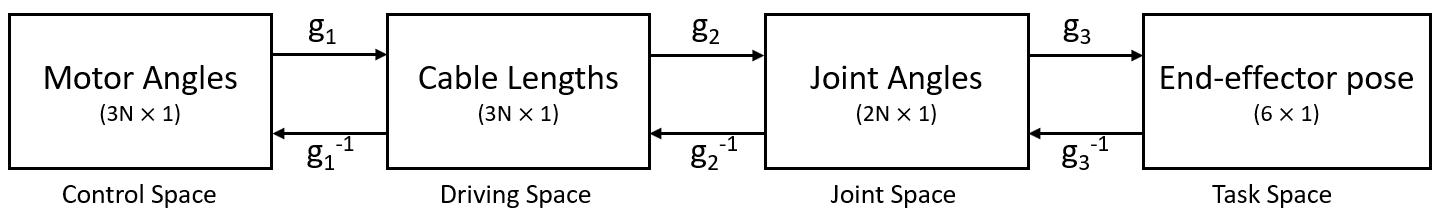
\includegraphics[width=\textwidth]{images/Kinematics-mapping.png}
	\caption{\textit{This picture shows the various mapping relationships required between different spaces to derive the relationship between the angle of rotation of the motor and the end-effector pose of the snake-arm}}
	\label{kinematic map}
\end{figure}
 
\subsubsection{Motor Angle of Rotation - Cable Length Kinematics}
The rotation of the motors at the base are transmitted as translational motion causing a change in length of the cable driving the robotic arm. For a given change in angle of rotation of the motor the change in cable length (the translational distance travelled) can be calculated as:
\begin{equation}
\label{eq:g1_inv}
\Delta L_{k} =\Delta \theta \times \frac{S}{168 \pi}
\end{equation}
where,
\begin{itemize}[label={--}]
	\item S = Pitch
	\item $\Delta L_{k}$ = Change in length of cable number k ($k \in [1,2,\ldots,3N]$) 
	\item $\Delta \theta$ = Angle of rotation of the motor
\end{itemize}

Equation \ref{eq:g1_inv} is the inverse kinematic relationship between the motor angle of rotation and cable length ($g_{1}^{-1}$ as per Figure \ref{kinematic map}). From this the forward kinematic relationship($g_{1}$ as per Figure \ref{kinematic map}) between the motor angle of rotation and cable length can be derived as:
\begin{equation}
\label{eq:g1}
\Delta \theta =\Delta L_{k} \times \frac{168 \pi}{S}
\end{equation}

\subsubsection{Cable Length - Joint Angle Kinematics}
To derive the relationship between the cable length and the joint angles, three reference frames $\{P_n\}$,$\{U_n\}$,$\{D_n\}$ must be defined at each universal joints as seen in Figure \ref{ref-frames}.

\begin{itemize}
	\item The reference frame $\{U_n\}$ is defined such that its origin ($O_U$) corresponds to the centre of the joint. $X_U$ is defined parallel to $\zeta_P$ and $Y_U$ is defined parallel to $\zeta_D$. $Z_U$ is then defined using right-hand thumb rule.
	\item The reference frame $\{P_n\}$ is defined such that its origin ($O_P$) corresponds to the centre of the proximal disk. $Z_P$ is normal to the proximal disc and $X_P$ is parallel to $\zeta_P$. $Y_P$ is then defined using right-hand thumb rule.
	\item The reference frame $\{D_n\}$ is defined such that its origin ($O_D$) corresponds to the centre of the distal disk. $Z_D$ is normal to the distal disc and $Y_D$ is parallel to $\zeta_D$. $X_D$ is then defined using right-hand thumb rule.
\end{itemize}
\begin{figure}[H]
	\centering
	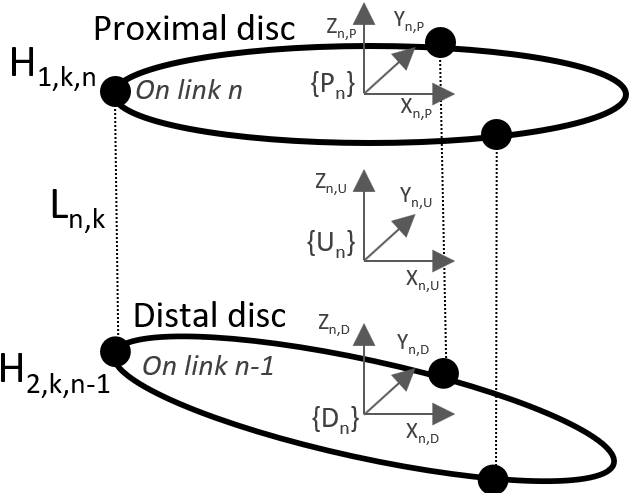
\includegraphics[width=0.5\textwidth]{images/Refrence_frames.png}
	\caption{\textit{This diagram shows the different reference frames that were defined}}
	\label{ref-frames}
\end{figure}
where, $\zeta_P$ and $\zeta_D$ represents the axis of rotation of the joint attached to the proximal and distal discs respectively.
This means that by definition we have the relationship: $O_{P,n}O_{U,n}=O_{U,n}O_{D,n}=2d$


The transformation matrix from $\{D_n\}$ to $\{P_n\}$ can be defined as: 
\begin{equation}
\begin{aligned}
^DA_P&=^DA_U \times ^UA_P \\ 
&= \begin{bmatrix}
\cos{\phi_{p,n}}&0&\sin{\phi_{p,n}}&d\sin{\phi_{p,n}}\\
\sin{\phi_{p,n}}\sin{\phi_{d,n}}&\cos{\phi_{d,n}}&-\sin{\phi_{d,n}}\cos{\phi_{p,n}}&-d\sin{\phi_{d,n}}\cos{\phi_{p,n}}\\
-\cos{\phi_{d,n}}\sin{\phi_{p,n}}&\sin{\phi_{d,n}}&\cos{\phi_{d,n}}\cos{\phi_{p,n}}&d+d\cos{\phi_{p,n}}\cos{\phi_{d,n}}\\
0&0&0&1\\
\end{bmatrix}\\
\end{aligned}
\end{equation}

As can be seen from Figure \ref{ref-frames} the length of the cable between 2 discs can be derived as:
\begin{equation}
\label{len_joints}
l_{k,n}= \lvert\lvert ^DA_P^PH_{1,k,n} - ^DH_{2,k,n-1}  \rvert\rvert
\end{equation}
such that,
\[
^PH_{1,k,n}=\begin{bmatrix}
r\cos{\delta_{k,n}}\\
r\sin{\delta_{k,n}}\\
0\\
\end{bmatrix} \hspace{4mm} ;\\
^DH_{2,k,n-1}=\begin{bmatrix}
r\cos{\delta_{k,n}}\\
r\sin{\delta_{k,n}}\\
0\\
\end{bmatrix} 
\]
The total length of the cable k can therefore be written as:
\begin{equation}
\label{len_total}
L_k= \sum_{n=1}^{N}l_{k,n}
\end{equation}
Therefore,  equations \ref{len_joints} and \ref{len_total} define the inverse kinematics relationship between the joint angles and the cable lengths ($g_{2}^{-1}$ as per Figure \ref{kinematic map}).

We know that for a given joint $n$, cables $3n-2$,$3n-1$ and $3n$ drive the joint. Therefore considering equation \ref{len_joints} to be a function of $\phi_p$ and $\phi_d$ we know there exists a relationship:
\begin{equation}
\begin{bmatrix}
l_{3n-2,n}\\
l_{3n-1,n}\\
l_{3n,n}\\
\end{bmatrix} =
\begin{bmatrix}
f_{3n-2}(\phi_{p,n},\phi_{d,n})\\
f_{3n-1}(\phi_{p,n},\phi_{d,n})\\
f_{3n}(\phi_{p,n},\phi_{d,n})\\
\end{bmatrix}
\label{function_of_l}
\end{equation}

From \ref{function_of_l} the differential equation can be derived as: 
\begin{equation*}
\begin{bmatrix}
dl_{3n-2,n}\\
dl_{3n-1,n}\\
dl_{3n,n}\\
\end{bmatrix} = J
\begin{bmatrix}
d\phi_{p,n}\\
d\phi_{d,n}\\
\end{bmatrix}
\label{differential_of_l}
\end{equation*}
where,\\
\indent J= Jacobian matrix of $[f_{3n-2}(\phi_{p,n},\phi_{d,n}),f_{3n-1}(\phi_{p,n},\phi_{d,n}),f_{3n}(\phi_{p,n},\phi_{d,n})]^{T}$ w.r.t $[\phi_{p,n},\phi_{d,n}]^{T}$

Therefore, the forward kinematics relationship between the joint angles and the cable lengths ($g_{2}$ as per Figure \ref{kinematic map}) can be numerically calculated as:
\begin{equation}
	 \begin{bmatrix}
	 \Delta \phi_{p,n}\\
	 \Delta \phi_{d,n}\\
	 \end{bmatrix}
	 = J^{+}
	 \begin{bmatrix}
	 \Delta l_{3n-2,n}\\
	 \Delta l_{3n-1,n}\\
	 \Delta l_{3n,n}\\
	 \end{bmatrix}
	\label{g2}
\end{equation}
where,\\
\indent $J^{+}$= Moore-Penrose pseudoinverse of J

\subsubsection{Joint Angle - End Effector Pose Kinematics}
To derive the joint angle - end effector pose kinematics a reference frame was define at each link for each DoF. The set of reference frames ${I_1},{I_1},{I_2},\ldots\\,{I_{2N}}$ is defined such that $Z_{i-1}$ of ${I_i}$ for the i\textsuperscript{th} rotation axis. Therefore, by definition the relationship between joint angles and the the rotation of the universal joints is given by,
\begin{equation}
 \begin{bmatrix}
\theta_{2n-1} \\
\theta_{2n} \\
\end{bmatrix}
= 
\begin{bmatrix}
(-1)^{n+1} \phi_{d,n}\\
\phi_{p,n}\\
\end{bmatrix}
\label{phi to theta}
\end{equation}
Therefore, $\Theta=[\theta_1,\theta_2,\theta_3,\ldots,\theta_2N]^T$
Using the above defined reference frames and the Denavit-Hartenberg parameters (D-H parameters) the homogenous transformation matrix any frame ${I_i}$ can be expressed in terms of the base reference frame as:
\begin{equation}
{}^{0}A_{i}=\prod_{j=1}^{i} {}^{j-1}A_j
\end{equation}
Therefore, the forward kinematics relationship between the joint angles and end-effector pose ($g_{3}$ as per Figure \ref{kinematic map}) can be numerically calculated as:
\begin{equation}
\dot{x_e}= J(\Theta)\dot{\Theta}
\label{g3}
\end{equation}
Then the inverse kinematics relationship between the joint angles and end-effector pose ($g_{3}^{-1}$ as per Figure \ref{kinematic map}) can be numerically calculated as:
\begin{equation}
\dot{\Theta}= J^{+}(\Theta)\dot{x_e}
\label{g3_inv}
\end{equation}

\subsection{Dynamic Modelling}
Although most literature details the kinematic model for a CDHRM and presents the experimental results for it, only very few and recent literature discusses the dynamic model of the CDHRM. For the dynamic model of a CDHRM \cite{RN30, RN51, mu_liu_xu_lou_liang_2019} were identified as good resources. \footnote{It must be noted that they are all papers that have been published quite recently and have very few forward citations.}

The following are the forces that are involved in the dynamic model of the CDHRM:
\begin{itemize}
	\item Cable Tension Forces
	\item Cable Contact Forces
	\item Link Gravitational Force
	\item Link Inertia Forces
	\item Adjacent Link Interaction Forces
\end{itemize}


\section{Progress to Date}
The kinematic model was identified, studied and its behaviour was verified for initial conditions (this is discussed in detail in the next chapter). However, since understanding the kinematic model and implementing it took longer than expected the dynamic equations could not be implemented. The literature discussing a dynamic model of a CDHRM have been identified and reading was done to understand the forces associated with the model. However, the equation has not been simulated yet.
%%%%%%%%%%%%%%%%%%%%%%%%%%%%%%%%%%%%%%

%%%%%%%%%%% MATHEMATICAL MODELLING %%%%%%%%%%%%%%%%%
\chapter{Implementation of the Model}
This chapter mainly discusses the work done towards the tasks associated with the Simulation and Modelling phase (second phase) of the project. However, since the first phase ran longer than expected, this affected the amount of progress achieved in tasks associated to simulation and modelling. Therefore, the Gantt chart was updated and Figure \ref{gc-2} shows the new version of the Gantt Chart for these tasks. 
\begin{figure}[h]
	\centering
	\includegraphics[width=\textwidth]{images/GC-chap3.png}
	\caption{\textit{Gantt Chart showing tasks associated to Simulation and Modelling Phase.}}
	\label{gc-2}
\end{figure}

\section{Implementation on Simulink}
The equations discussed in the previous chapter were implemented on Simulink as discussed in the following sub-sections.
The following values were assigned to the constants in the equations for simulation:
\begin{table}[h!]
\centering
\begin{tabular}{|c|c|c|}
	\hline
	\textbf{Description} &\textbf{Variable} & \textbf{Value} \\
	\hline
	Number of joints & N & 9\\
	Distance between adjacent links & d & 11.5mm\\
	Length of a link & a & 140 mm\\
	Radius to hole positions & r & 20.5mm\\
	Pitch & S & 8mm\\
	\hline
\end{tabular}
\caption{Values used for the constants in the model}
\label{params_table}
\end{table}

\subsection{Motor Angle of Rotation - Cable Length Kinematics}
The forward and inverse kinematics equation for these are defined  by equations \ref{eq:g1} and \ref{eq:g1_inv} in the previous chapter. Amongst the other equations, the mapping between motor angle of rotation and cable length is the most straight forward as the relationship is of linear proportionality. The equations were implemented directly using Simulink blocks as shown in Figure \ref{g1} and \ref{g1_inv}. To compute the change in angle or change in length the memory clock was used to get the value of the variable computed during the previous time step.
\begin{figure}[H]
	\centering
	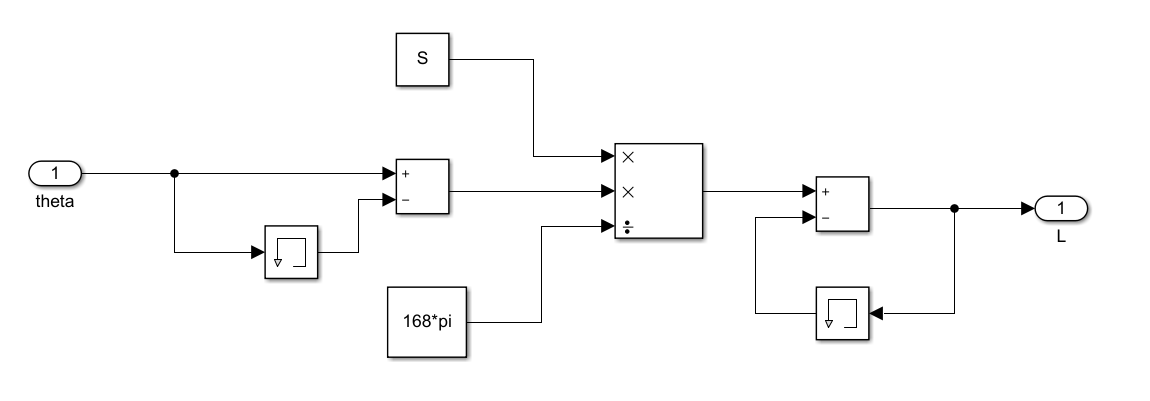
\includegraphics[width=\textwidth]{images/g1.png}
	\caption{\textit{Implementation of Motor Angle of Rotation - Cable Length Forward Kinematics }}
	\label{g1}
\end{figure}

\begin{figure}[H]
	\centering
	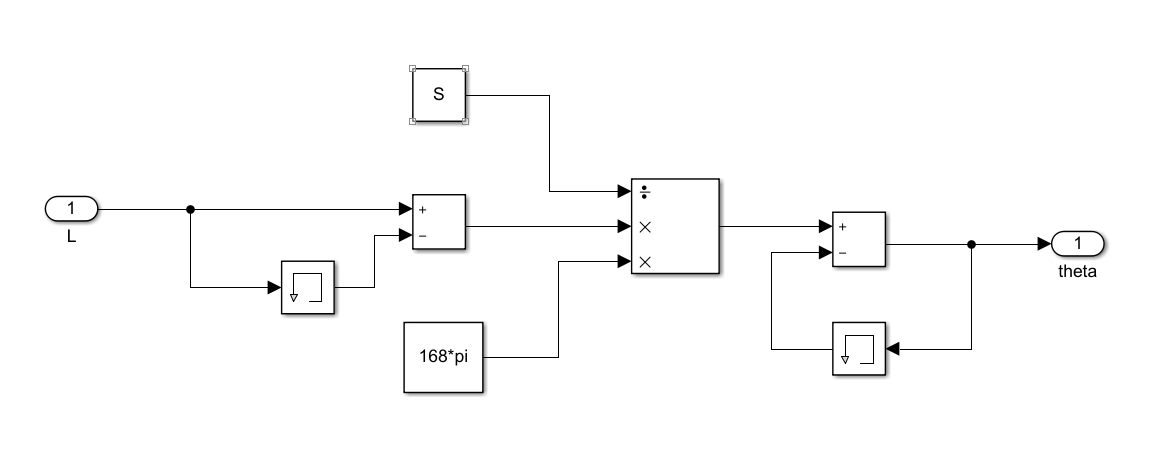
\includegraphics[width=\textwidth]{images/g1_inv.png}
	\caption{\textit{Implementation of Motor Angle of Rotation - Cable Length Inverse Kinematics }}
	\label{g1_inv}
\end{figure}


\subsection{Cable Length - Joint Angle Kinematics}

The inverse kinematics solution given by \ref{len_joints} ($g_2^{-1}$) is easily achievable as a simple matrix multiplication. This was therefore written as single MATLAB function block for simplicity.

Since calculating the Jacobian required the use of $\phi_{p,n}$ and  $\phi_{d,n}$ it was not possible for the equation to be directly implemented. Instead a numerical iterative method was used which assumed the value of  $\phi_{p,n}$ and  $\phi_{d,n}$ (both set initially at 0 rad) and then the value of $l_{n.k}$ was iteratively calculated till difference between the desired cable length and calculated cable length was less than the fixed error tolerance ($\epsilon$). This was set as $\epsilon=0.001$. If the number of iterations exceed 10000, the loop is exited and the input is considered to have no solution. Figure \ref{fc1} shows the flow chart depicting the numerical iteration process used to compute the forward kinematics solution for cable length - joint angle mapping.
\begin{figure}[H]
	\centering
	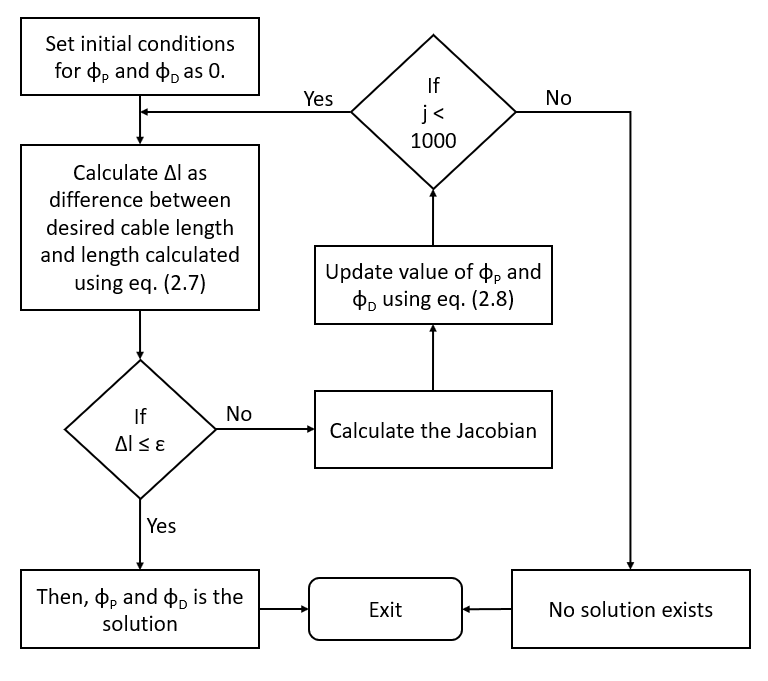
\includegraphics[width=0.75\textwidth]{images/Iteration_1.png}
	\caption{\textit{Numerical iteration process adopted to calculate the solution of the forward kinematics of for cable length - joint angle mapping}}
	\label{fc1}
\end{figure}
The code associated to this sub-section can be found in \ref{appendix:c-a}.

\subsection{Joint Angle - End Effector Pose Kinematics}

The forward kinematics of this mapping given by equation \ref{g3} ($g_3$) can be easily implemented by calculating the associated Jacobian as shown in the adjacent Figure \ref{g3-fig}.
\begin{figure}[H]
	\centering
	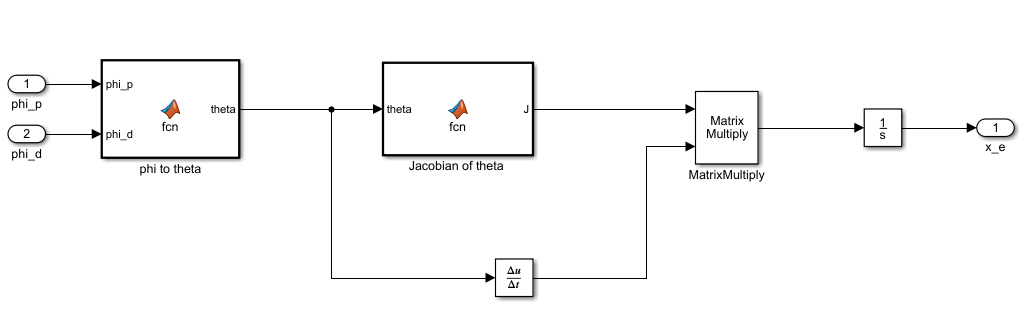
\includegraphics[width=\textwidth]{images/g3.png}
	\caption{\textit{Simulink model made to implement the forward kinematics of {Joint Angle - End Effector Pose}}}
	\label{g3-fig}
\end{figure}

For solving the inverse kinematics for the joint angle - end effector pose a numerical iterative process similar to the one followed for implementation of the forward kinematics relationship in the previous sub-section is adopted. Figure \ref{fc2} shows the flow chart depicting the numerical iteration process used to compute the forward kinematics solution for cable length - joint angle mapping.
\begin{figure}[H]
	\centering
	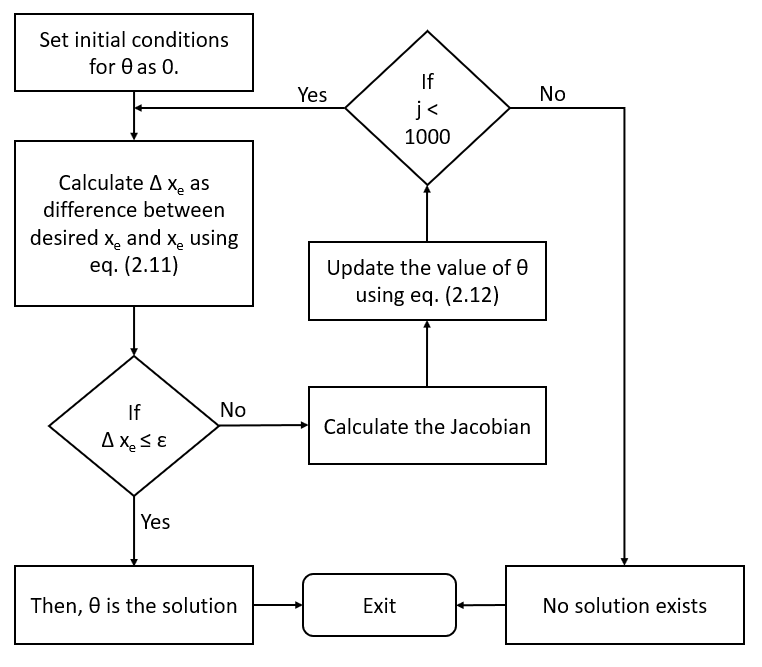
\includegraphics[width=0.75\textwidth]{images/Iteration_2.png}
	\caption{\textit{Numerical iteration process adopted to calculate the solution of the forward kinematics of for joint angle - end effector pose mapping}}
	\label{fc2}
\end{figure}

\section{Verifying the model}
To verify the behaviour of the model, the equations were cross-validated using the known initial conditions. The output from the forward kinematic blocks was given as input to the inverse kinematics block to check if input of the former is at least approximately equal to that of the inverse kinematics block.
Figure \ref{motor_verify} to Figure \ref{end_verify} show the separate arrangements for the three individual kinematic mapping relationships.
\begin{figure}[H]
	\centering
	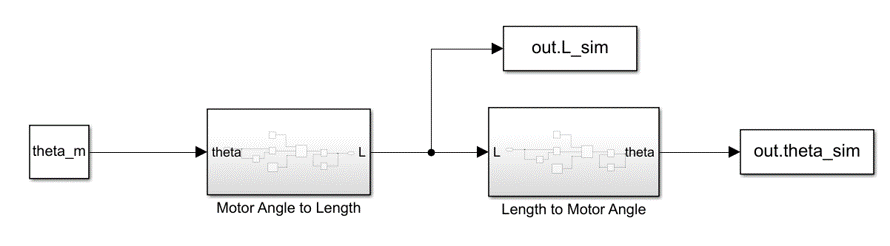
\includegraphics[width=\textwidth]{images/length_to_motor_angle_verify.png}
	\caption{\textit{Cross-validation model for Motor Angle of Rotation - Cable Length Kinematics }}
		\label{motor_verify}
	\end{figure}
\begin{figure}[H]
	\centering
	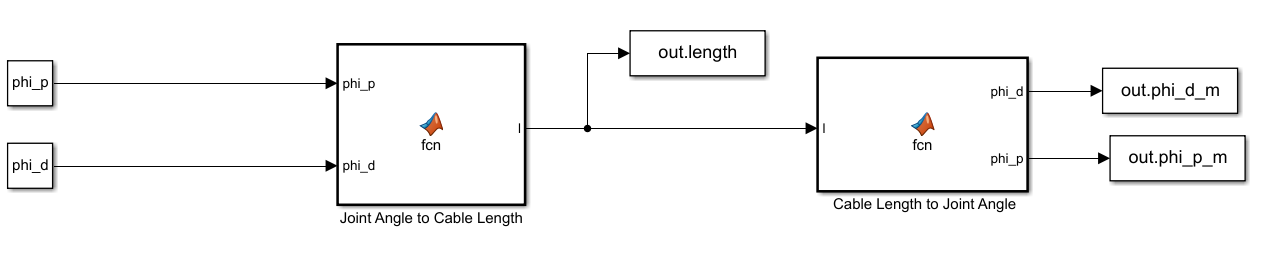
\includegraphics[width=\textwidth]{images/cable_to_angle_verify.png}
	\caption{\textit{Cross-validation model for Cable Length - Joint Angle Kinematics}}
		\label{length_verify}
	\end{figure}
\begin{figure}[H]
	\centering
	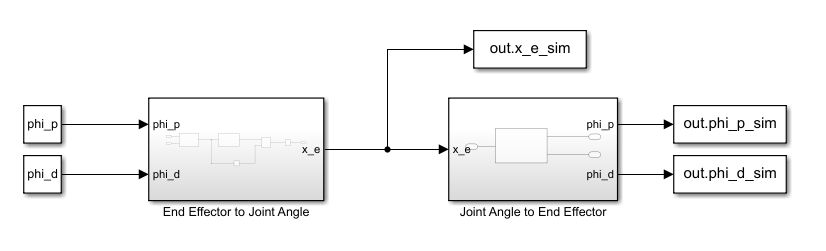
\includegraphics[width=\textwidth]{images/joint_to_end_verify.png}
	\caption{\textit{Cross-validation model for Joint Angle - End Effector Pose Kinematics }}
		\label{end_verify}
	\end{figure}

The outputs that were saved to workspace were then compared separately for cross-validation and the results obtained were equal on both sides as expected. 
 
\section{Progress to Date}
Implementing the mathematical model and cross-validating the equations was the first step towards building and testing the mathematical model. Now the next step is to use a simple PD controller to combine the several levels of the kinematic model and to test the baseline/initial results for tracking error of the given system.

%%%%%%%%%%%%%%%%%%%%%%%%%%%%%%%%%%%%%%

%%%%%%%%%%% CONCLUSIONS %%%%%%%%%%%%%%%%%
\chapter{Summary of Difficulties and Issues}
\section{List of Difficulties and Issues} 
During the project work undertaken last term the following difficulties occured:
\begin{itemize}
	\item Preparatory phase took longer than expected as a result of which desired progress could not be achieved in tasks related to the Simulation and Modelling Phase. The Gantt Chart has now been updated to reflect the extra time required for other tasks. However, kinematic model is well-known. Understanding the kinematic model took more time than expected as it took some time to identify necessary background reading required to understand the kinematic model.
	\item Not many sources discuss the dynamic model in detail. However, some papers were identified that were published quite recently and hence has no forward citations.
	\item While it was expected that Term 1 would be more relaxed than Term 2 in terms of coursework and assessments from other modules, it turned out that there were several submissions throughout the term which considerably reduced the time that could be spent on the project. This should not be the case next term since all modules chosen are 100\% exam modules.
\end{itemize}
\section{Failure Risk Assessment}
The project mainly involves modelling of a dynamic system and analysing its behaviour under control system configurations. Therefore, with respect to this project, failure can be mainly thought of as \textbf{not being able to simulate the behaviour of the real dynamic system using the mathematical model chosen} or \textbf{not being able to obtain expected tracking of the reference parameters}.

Several factors can cause these failures, therefore to tackle such unexpected behaviour and/or arbitrary results, an iterative method is used for testing and improvement of the results. From a very early stage (as can be seen in the Gantt Chart), the results will be compiled, understood and analysed to understand how improvements can be made. Necessary changes will be then incorporated, and this process will be repeated till desired tracking of parameters is achieved. Each iteration may involve improvements made through educated trial and error methods and/or experiments. 

Iterations may also involve major changes to the simulation model. If after several attempts desired results could not be obtained, then different control system configurations will be attempted and changes supporting improved results will be adopted. To make it easier, during literature review possible variations of the mathematical model will be noted and recorded so that if the mathematical model fails to behave as expected one of the simpler options could be implemented instead.

Currently, the robotic snake-arm has been identified as a continuum robot however, if this approach fails to represent the behaviour of the model, then an alternative model that represents the system will be identified or else the last resort would be fall back on the simplified option for the mathematical model which is the approach of a simplifying the snake-arm as a modular robotic arm with several rigid links of a fixed length. The modular “vertebrae-like” model would still simulate the behaviour of the arm even though the number of degrees of freedom of the system might reduce significantly.

Additionally, the weekly project tutorials with the project supervisor will also help give new perspectives and ideas on how the results can be improved.

\section{Safety Risk Assessment}
Since the project does not include any tasks involving hardware or use of laboratory equipment and machinery, the risks associated are only those around working on a computer. Some of the main safety risks associated to working on a computer have been identified as:
\begin{itemize}
	\item  	\textbf{Eyestrain:} Long hours of looking into a screen especially with incorrect screen settings and in a room with poor/intrusive lighting conditions can lead to eyestrain and headache related to it. \\ \\
	\textbf{Control measures:}
	\begin{itemize}
		\item Ensure that the screen settings are suitable for the lighting conditions of the room. The contrast, brightness and colours of the screen must be easy on the eyes.
		\item Face your screen away from intrusive light or glare. This can be avoided by facing it away from windows, bulbs and bright light in the room.
		\item Ensure that the screen is clean.
		\item Make sure that while reading, the screen in zoomed in sufficiently so that the letters are large enough to be read from a comfortable position.
		\item Ensure that the text on the screen is sharp and in focus. The screen should not flicker, and the text must not appear to be moving.
		\item Give your eyes a break from looking into the screen by looking into the distance from time to time.
	\end{itemize}
	\item \textbf{Poor Posture:} Poor posture while sitting at a work station can lead to discomfort from aches, backpain etc. and may even cause injury. Poor posture may even be caused due to poor workstation set up.\\ \\
	\textbf{Control measures:}
	\begin{itemize}
		\item Ensure that you are sitting upright with your back positioned comfortably on the backrest of the chair. Sit close to the desk to prevent leaning forward uncomfortably.
		\item Ensure that your eyes are at the same height as the top of the screen.
		\item Take short and frequent breaks and change position if possible.
	\end{itemize}
	\item \textbf{Repetitive movements:} Poorly designed workstations or uncomfortable working postures might lead to repetitive strained movements and can cause repetitive strain injuries. \\ \\
	\textbf{Control measures:}
	\begin{itemize}
		\item Take short and frequent breaks and if possible, stretch and change position.
		\item Make sure there is space under the desk to move legs.
		\item Ensure that the workstation layout does not contribute to repetitive strained movements. Choose a comfortable space.
		\item Position the mouse such that it is within easy reach and can be held with a straight wrist
		\item When not typing use the space in front of keyboard to rest your wrists and hands.
		\item Do not overstrain muscles by overstretching fingers when typing or holding onto the mouse with a tight grip.
		\item Sit upright and close to the desk to reduce working with the mouse with your arm stretched.
	\end{itemize}
	\item \textbf{Tripping:} When working in computer labs or study spaces there is a risk of tripping over objects or slipping on spillages. \\ \\
	\textbf{Control measures:}
	\begin{itemize}
		\item Be mindful and careful of obstructions on the floor/walkways even in rooms that you are used to working in. Avoid walking around carelessly or looking into the screen of the computer.
		\item Inform the responsible management if any major obstruction with potential risk is noticed. This may include damaged floors, trailing cables, inadequate housekeeping, incorrect lighting levels etc.
	\end{itemize}
	\item 	\textbf{Poor lighting conditions:} Poor lighting conditions refers to both insufficient lighting as well as excessive lighting of a room. Poor lighting conditions may cause headaches or sore eyes.\\ \\
	\textbf{Control measures:}
	\begin{itemize}
		\item Control the lighting in the room suitably.
		\item Adjust the blinds to control natural light levels or to avoid glare on screens.
	\end{itemize}
	\item \textbf{Lone working:} When working alone in the office there is risk of injuries, emergencies etc. with inadequate provision for help.\\ \\
	\textbf{Control measures:}
	\begin{itemize}
		\item Avoid non-routine working.
		\item Be aware of the risks and precaution associated to the work undertaken.
		\item Have the information and knowledge of how to deal with emergencies
	\end{itemize}
\end{itemize}

The above-mentioned risks are the main risks associated to working on a computer. A more exhaustive list of risks, including ones that are very unlikely, were submitted via RiskNET. The approved risk assessment report can be found in Appendix \ref{appendix:b}.	


\section{Additional Work to Complete Goals}
The main additional work left to complete the goals of the project involves the last two objectives as stated in section \ref{objectives}. Since a mathematical model has now been implemented and tested, the next tasks are: 
\begin{itemize}
	\item Implement the dynamic model equations and integrate that with the kinematic model.
	\item Try different simple control strategies (mainly PD control and PD+feedforward control) and record a baseline result for the tracking error of the end-effector pose. Then, try improving the performance by minimising the tracking error.
	\item Analyse the robustness of the control system by running experiments with varied physical parameters (mainly by changing mass of link N and by introducing disturbances).
\end{itemize}
\begin{figure}[H]
	\centering
	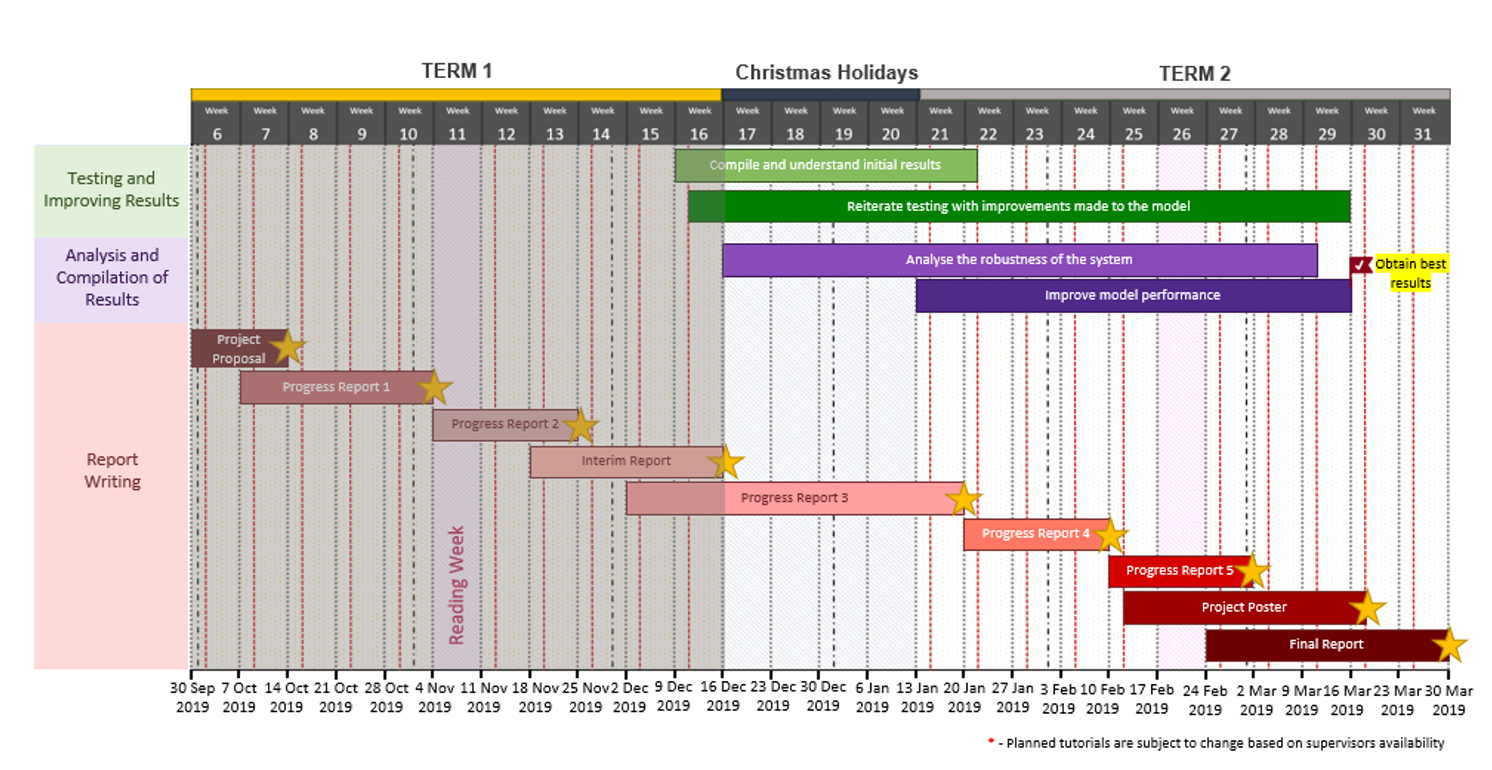
\includegraphics[width=\textwidth]{images/gc-chap4.png}
	\caption{\textit{Gantt Chart showing tasks associated with the additional work to be done to complete the goals of the project}}
	\label{gc-4}
\end{figure}
Figure \ref{gc-4} shows the updated Gantt Chart for the additional work required to be done. 

The updated Gantt Chart has been added with a clearer picture for the Gantt Charts from the previous sections, to the next page.
\pagebreak
\label{UpdatedGC}
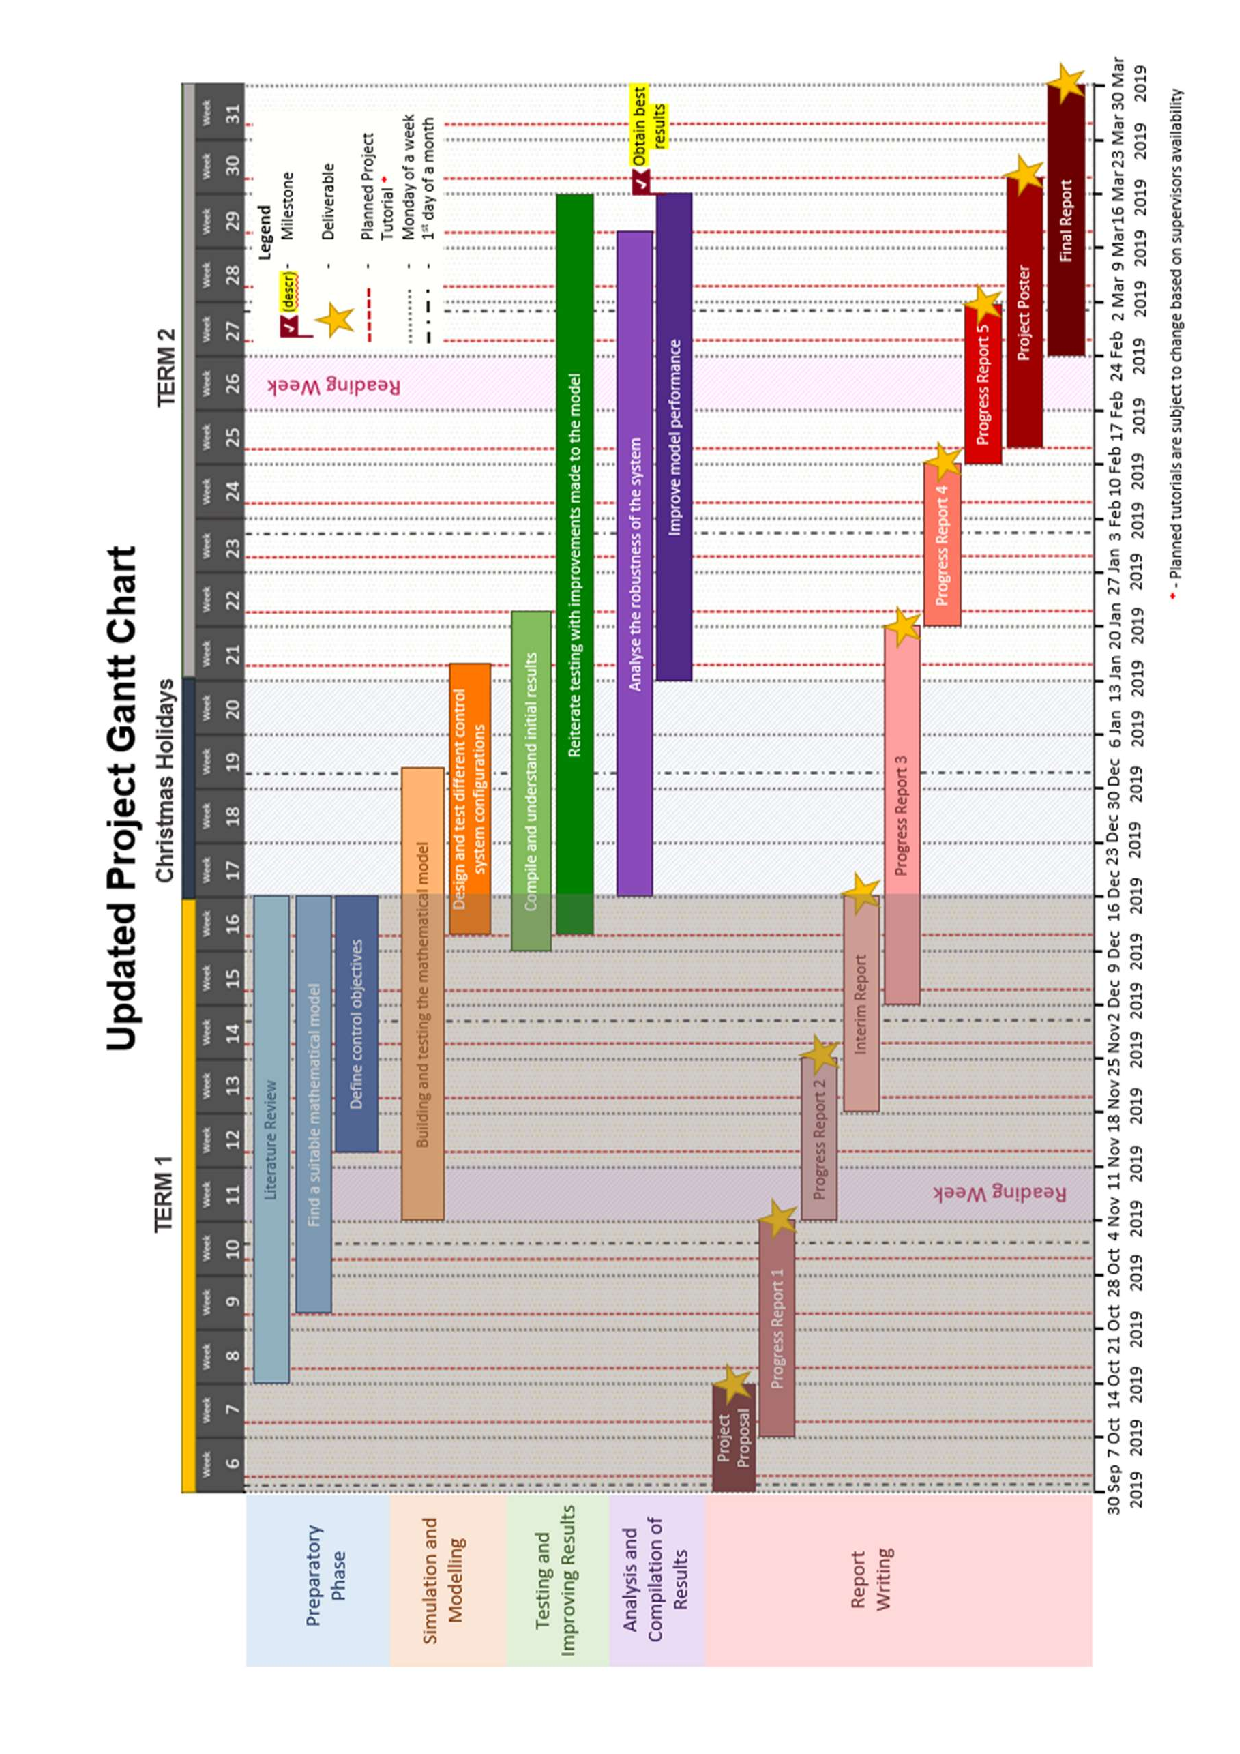
\includepdf[page=-]{files/Gantt Chart - Updated}


%%%%%%%%%%%%%%%%%%%%%%%%%%%%%%%%%%%%%%

%%%%%%%%%%% APPENDIX %%%%%%%%%%%%%%%%%
\begin{appendices}
	\chapter{Project Gantt Chart {\normalsize (as submitted with proposal)}}
	This appendix discusses the Project work plan and Gantt Chart as submitted in the project proposal.
	The project will mainly have four phases - \textit{Preparatory phase, Simulation and Modelling, Testing and Improving results} and \textit{Analysis and Compilation of Results}
	\begin{itemize}
		\item \textbf{Preparatory Phase:} The first month and a half will involve preparatory phase during which through literature review several suitable mathematical models will be identified and the model that best represents the physical snake-arm will be implemented. During this phase the control objectives of the snake arm will also be clearly investigated and will be defined mathematically.
		Work undertaken over summer proved that the approach of mimicking a biological snakebot to improve reach and span of the robot will not be suitable, as controlling such a snakebot poses a lot of challenges. Even though extensive research over the years have led to improved results, the level of accuracy of the tracking of the controlled variable is lower than what is required for a task like air wing inspection. The risk of a snake-arm making contact with the structures due to incorrect path following can be very unsuitable for this scenario. Also, given that the OC Robotics snake-arm is more like a tethered continuum robot moving in free space, the viscous friction model adopted by most authors to describe the dynamic model of a wheel-less ground-hugging robot snakebot won’t be suitable. Therefore, the initial approach when modelling the snake-arm the concept of continuum robots may be used the most.
		\item \textbf{Simulation and Modelling:} The next phase of the project will then involve implementing the mathematical model, simulating the control system on Simulink and obtaining the initial results. The tracking error of the parameters (specially speed, position and orientation) will be analysed and efforts will be made to improve these results. It is expected that at this stage, an iterative testing method would be adopted to improve the model until desired tracking accuracy is obtained.
		\item \textbf{Testing and Improving Results:} From the start of the second phase to the end of the project, results will be improved and tested iteratively until desired results are achieved. Although this has been specified as a separate phase it represents the steps that are part of the second and the last phase. 
		\item \textbf{Analysis and Compilation of Results:} Once satisfactory results are obtained; the final phase of the project will focus on testing the robustness of the system in varied conditions. It is expected that the payload attached to the head will change depending on the optical metrology technique for which it is being used. Further, it might be performing measurements in environments where external disturbances are no longer negligible. So, for these scenarios, tests will be performed to analyse the robustness of the system to these disturbances.
		Results obtained will be reported systematically and periodically through progress reports that are roughly due once in every three weeks since the start of the project.
	\end{itemize}
	
	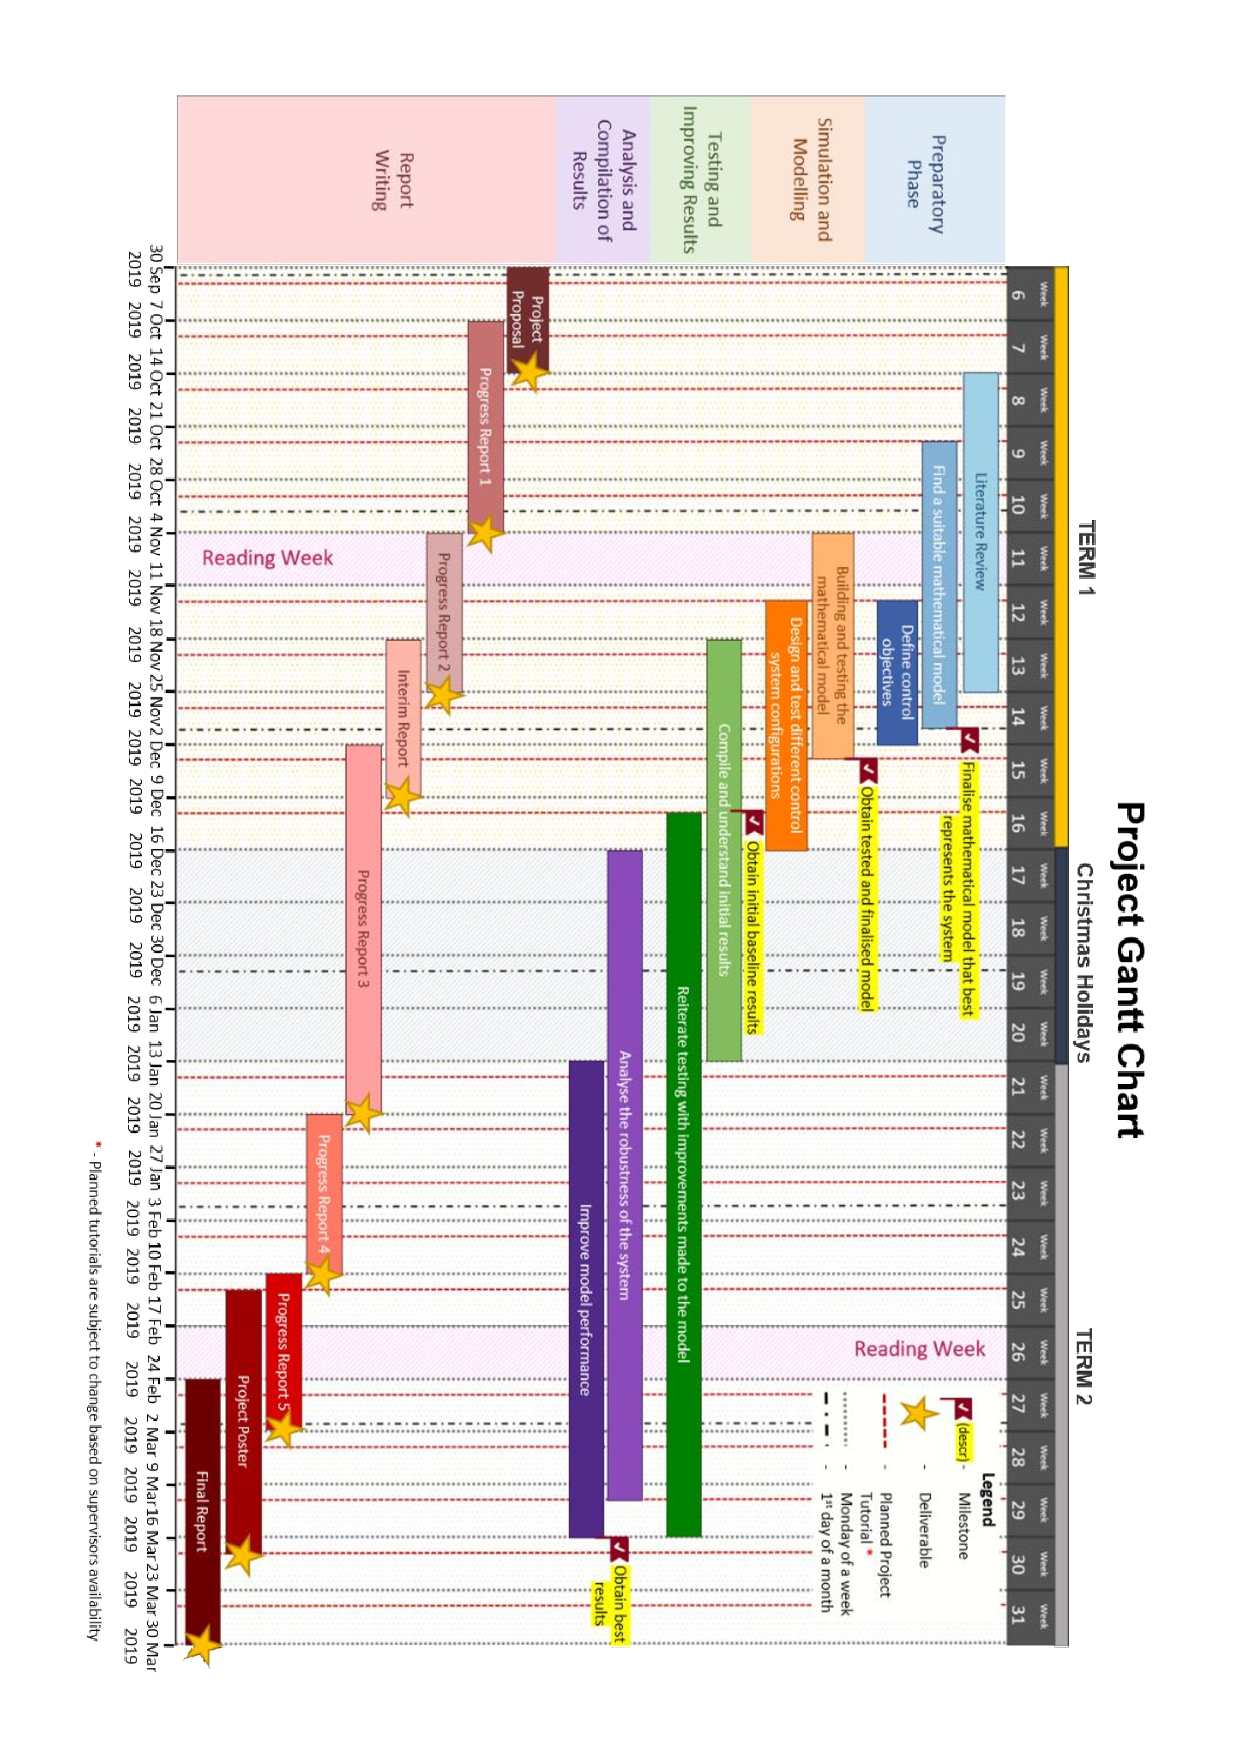
\includepdf[page=-]{files/Gantt Chart}
	\chapter{Risk Assessment}
	\label{appendix:b}
	The following hazards were identified through the risk assessment:
	\begin{itemize}
		\item Eyestrain
		\item Poor posture
		\item Repetitive movements involved with working on a computer
		\item Tripping over objects
		\item Poor lighting conditions
		\item Lone working
		\item Fire
		\item Contact with electricity
		\item General Welfare
	\end{itemize}
	The following pages includes a summary of the approved risk assessment generated using RiskNET.\\
	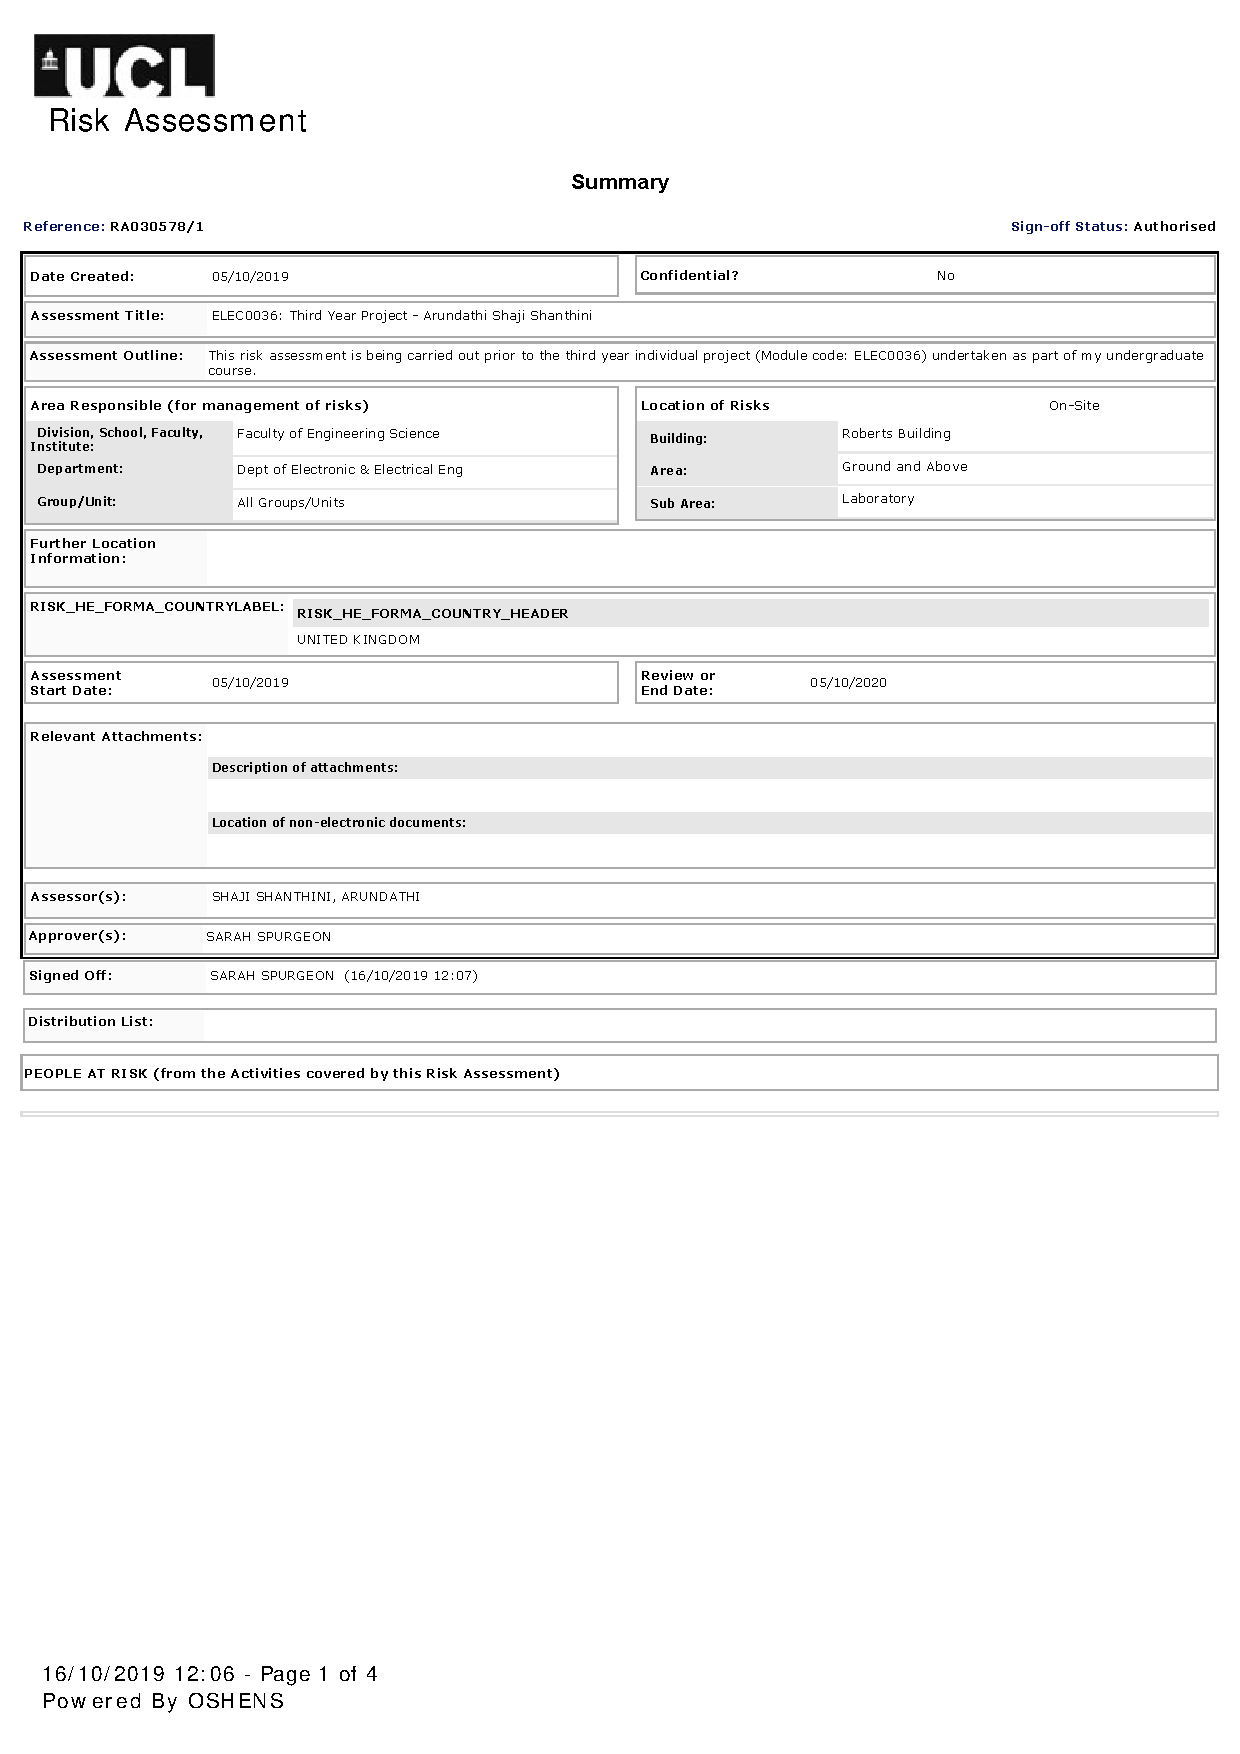
\includepdf[page=-]{files/Risk Assessment}
	\chapter{MATLAB Code}
	\label{appendix:c}
	\section{Cable Length - Joint Angles Mapping}
	\label{appendix:c-a}
	\subsection{Cable Length to Joint Angles}
	\lstinputlisting[language = Matlab]{code/length_to_angle.m}
	\subsection{Joint Angles to Cable Length}
	\lstinputlisting[language = Matlab]{code/angle_to_length.m}
	
	\section{Joint Angles - End-effector position Mapping}
	\label{appendix:c-b}
	\subsection{Joint Angles to End-effector position}
	\lstinputlisting[language = Matlab]{code/joint_to_end.m}
	\subsection{End-effector position to Joint Angles}
	\lstinputlisting[language = Matlab]{code/end_to_joint_jacobian.m}
	\lstinputlisting[language = Matlab]{code/end_to_joint_theta.m}
\end{appendices}
%%%%%%%%%%%%%%%%%%%%%%%%%%%%%%%%%%%%%%

\bibliographystyle{IEEEtran}
\bibliography{references}

\end{document}